\documentclass[runningheads]{llncs}
\usepackage[spanish]{babel}
\usepackage[utf8]{inputenc}
\usepackage[T1]{fontenc}
\usepackage{graphicx}
\usepackage{amsmath}
\usepackage{amssymb}
\usepackage{wrapfig}
\usepackage{listings}
\usepackage[T1]{fontenc}  % Para mejor codificación tipográfica (opcional pero recomendado)
\usepackage{float}

\lstset{
  breaklines=true,
  breakatwhitespace=true,
  basicstyle=\small\ttfamily  % Acá cambiás el tamaño de fuente y el tipo
}

\renewcommand{\lstlistingname}{Programa}

\begin{document}

\title{Análisis semántico durante el proceso de compilación}

\author{
    Florencia Luciana Brunello, 
    Andrés Valentino Ferrero, 
    Julieta Paola Storino
}

\authorrunning{Brunello, Ferrero, Storino.}

\institute{
    Facultad de Matemática, Astronomía, Física y Computación\\
    Universidad Nacional de Córdoba
}

\maketitle

\begin{abstract}
En este informe presentaremos una descripción general de la etapa de análisis semántico en el proceso de compilación, basado en el libro \textit{"Modern Compiler Implementation in ML"} \cite{1}. Dicho texto expone técnicas, estructuras de datos y algoritmos fundamentales para la implementación de compiladores mediante el desarrollo progresivo de un compilador para \textit{Tiger}, un lenguaje de programación didáctico de la familia de Algol creado por el autor. El compilador se implementa utilizando ML, un lenguaje funcional con tipado estático, estricto y modular que facilita la representación de las estructuras internas del compilador.
\end{abstract}

\section{Introducción}
Un compilador es una herramienta fundamental en el proceso de transformación del código fuente en ejecutable \cite{2}. Este proceso se organiza en una secuencia de fases (\textit{Figura 1}), que permiten descomponer y analizar progresivamente el programa. Antes de llegar a la etapa del análisis semántico, es necesario atravesar las siguientes fases previas:
\begin{enumerate}
    \item \textbf{Lex}: divide el código fuente en unidades léxicas o \textit{tokens}.
    \item \textbf{Parse}: analiza la estructura sintáctica del programa.
    \item \textbf{Parsing Actions}: construye los nodos del \textit{Abstract Syntax Tree} (AST) correspondientes a cada frase analizada.
\end{enumerate}

\begin{figure}[H]
    \centering
    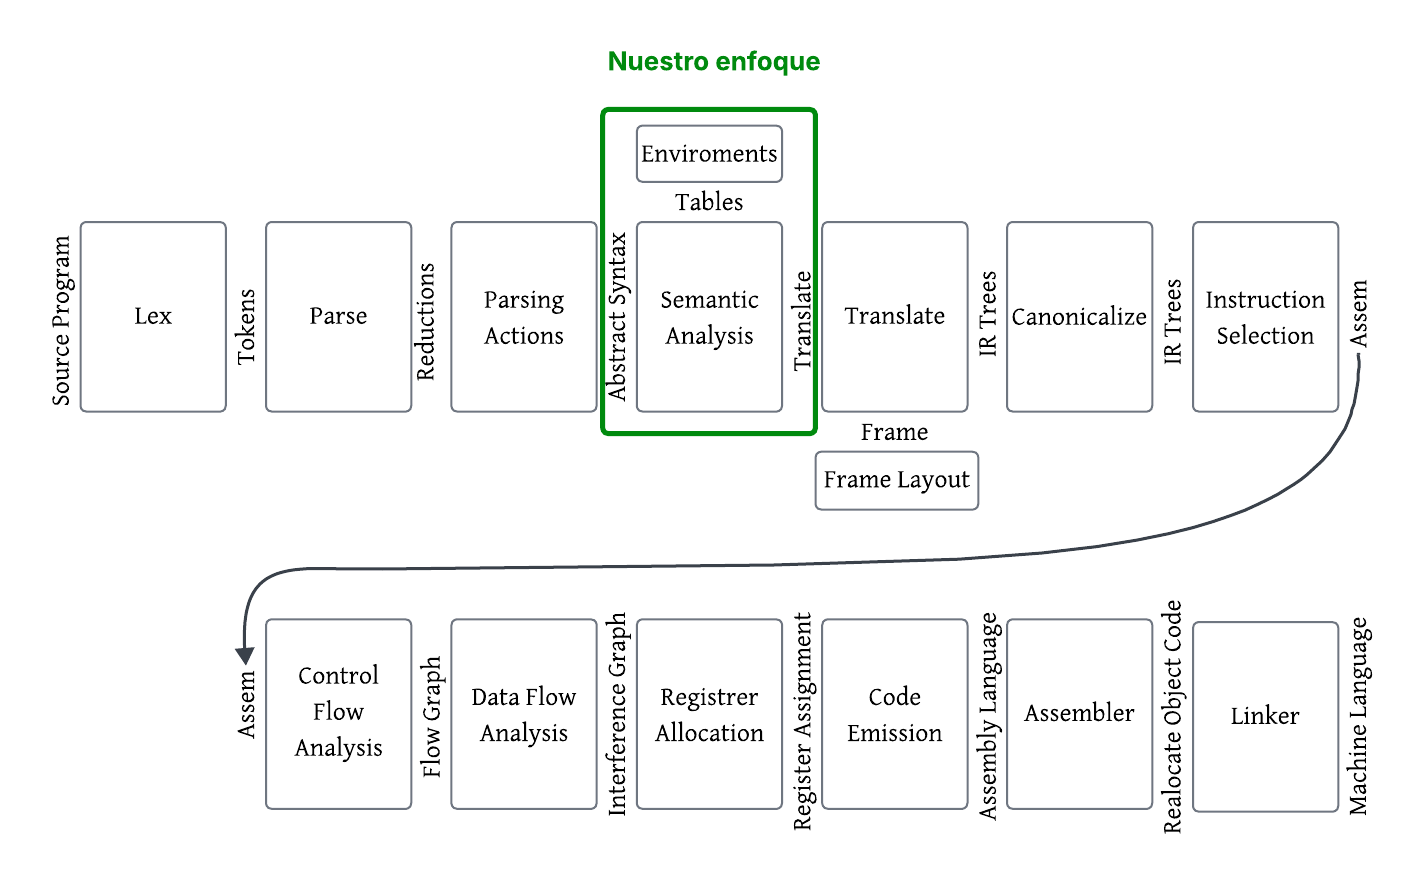
\includegraphics[width=7.5cm]{fases-compilador.png}
    \caption{Fases de un compilador y sus interfaces.}
    \label{fig:fases-compilador}
\end{figure}

\section{Tablas de Símbolos}
El análisis semántico de un compilador se caracteriza principalmente por el uso de \textit{symbol tables} o también llamados \textit{environments}. Un environment es un conjunto de bindings (asociaciones) denotadas por $\mapsto$, que vinculan identificadores de tipos, variables y funciones a sus respectivos tipos y ubicaciones. Por otro lado, cada variable tiene un \textit{scope} (alcance) donde es visible. Cada variable local tiene un scope en el cual puede ser referenciada. Una vez finalizado el alcance de esta, la asociación a la variable es descartada del environment.

El manejo de environments puede implementarse con un estilo \textit{imperativo} o \textit{funcional}, independientemente del lenguaje que se esté compilando o del estilo de implementación del compilador.

\subsection{Tablas Imperativas de Símbolos}
En las tablas imperativas de símbolos se mantiene un único environment global y una \textit{undo-stack} con suficiente información para deshacer las actualizaciones. Cuando se añade un símbolo al environment, actualizando este último, también se agrega a la pila. Al final de un scope, los símbolos extraídos tienen su última asociación eliminada, restaurando la asociación anterior.

Debido a que un programa puede tener muchos identificadores distintos, las tablas de símbolos deben permitir búsquedas eficientes. Es por esto que los environments suelen implementarse utilizando \textit{tablas hash con encadenamiento externo}, donde las colisiones se resuelven mediante listas enlazadas en cada bucket. 

De esta manera, la operación $\sigma_{i+1} = \sigma_i + {a \mapsto \tau}$ se implementa insertando $\tau$ en la tabla hash con la clave $a$, siempre que $a$ no haya sido definida previamente. En caso contrario, se crea un \textit{bucket} que apunta al valor anterior, de modo que, al buscar la variable, se obtenga $\tau$ como valor actual.

\subsection{Tablas Funcionales de Símbolos}
En las tablas funcionales de símbolos cada actualización produce una nueva versión del environment, manteniendo inmutable la anterior. Al finalizar un scope, simplemente se descarta la versión extendida, recuperando automáticamente el environment anterior sin necesidad de realizar operaciones de deshacer.

Las tablas hash, diseñadas para mutabilidad no son ideales en entornos funcionales, donde se requieren actualizaciones no destructivas. En cambio, se utilizan \textit{árboles de búsqueda binaria} que permiten actualizaciones inmutables y eficientes. Además, cada nueva versión de la estructura comparte nodos con la versión anterior, evitando copias completas.

De esta manera, la operación $\sigma_{i+1} = \sigma_i + \{a \mapsto \tau\}$ no altera la tabla original, sino que construye una nueva versión que extiende $\sigma_i$ con la asociación $a \mapsto \tau$. Internamente, esto se implementa compartiendo la estructura previa y enlazando el nuevo par $(a,\tau)$ al nodo raíz de la tabla. Así, al consultar la variable $a$ en $\sigma_{i+1}$, se obtiene directamente $\tau$, mientras que $\sigma_i$ permanece intacta para usos posteriores o para restaurarse automáticamente al salir de un \textit{scope}.

\subsection{Tabla de Símbolos en el compilador Tiger}
En el compilador de Tiger, los entornos se implementan con un estilo funcional. El módulo \texttt{SYMBOL} define una interfaz polimórfica para manejar entornos. Por cuestiones de eficiencia en las búsquedas, cada \texttt{string} es convertido a un \texttt{symbol}. Las tablas (\texttt{'a table}) permiten asociar símbolos con diferentes tipos de información (valores, tipos, etc.), donde \texttt{enter} añade asociaciones (creando una nueva tabla) y \texttt{look} permite buscar \texttt{el binding} de un símbolo.

\begin{lstlisting}[language=ML, caption={Firma del módulo SYMBOL}, captionpos=b]
signature SYMBOL =
sig
   eqtype symbol
   val symbol : string -> symbol
   val name : symbol -> string

   type 'a table
   val empty : 'a table
   val enter : 'a table * symbol * 'a -> 'a table
   val look  : 'a table * symbol -> 'a option
end
\end{lstlisting}

Internamente, cada símbolo se representa como un par \texttt{(string $\times$ int)}. Un contador llamado \texttt{nextsym}, junto con una tabla hash, se encarga de que cada entero sea único a cada cadena. Esta representación facilita comparaciones más eficientes y permite utilizar \texttt{IntBinaryMap} para implementar las tablas.

\begin{lstlisting}[language=ML, caption={Implementación de SYMBOL}, captionpos=b]
 structure Symbol :> SYMBOL =
 struct
   type symbol = string * int

   exception Symbol
   val nextsym = ref 0
   val hashtable : (string,int) HashTable.hash_table =
     HashTable.mkTable(HashString.hashString, op =)
                        (128, Symbol)

   fun symbol name =
     case HashTable.find hashtable name
       of SOME i => (name, i)
        | NONE => let val i = !nextsym
                  in nextsym := i+1;
                    HashTable.insert hashtable (name, i);
                    (name, i)
                  end

   fun name(s, n) = s

   type 'a table = 'a IntBinaryMap.map
   val empty = IntBinaryMap.empty
   fun enter(t: 'a table, (s, n): symbol, a: 'a) =
        IntBinaryMap.insert(t, n, a)
   fun look(t: 'a table, (s, n): symbol) =
        IntBinaryMap.look(t, n)
 end
\end{lstlisting}

\section{Asociaciones para el compilador Tiger}
En el lenguaje Tiger existen dos \textit{namespaces}: uno para los tipos y otro para las variables y funciones. Un identificador de tipo se asocia a un elemento del tipo \texttt{Types.ty}, definido en el módulo \texttt{Types}, el cual representa la estructura de tipos del lenguaje.

\begin{lstlisting}[language=ML, caption={Definición del módulo Types}, captionpos=b]
    structure Types = 
    struct 
        type unique = unit ref
        datatype ty = INT
                    | STRING
                    | RECORD of (Symbol.symbol * ty) list * unique
                    | ARRAY of ty * unique
                    | NIL
                    | UNIT
                    | NAME of Symbol.symbol * ty option ref
    end
\end{lstlisting}

También define dos clases de tipos: los primitivos (\texttt{int} y \texttt{string}) y los tipos construidos, que pueden ser \texttt{record} o \texttt{array} de otro tipo. Los records están compuestos por campos con nombre y tipo. Como cada expresión de tipo record representa una construcción distinta, Tiger los distingue mediante un valor especial llamado \texttt{unique}.

\subsection{Environments}
El tipo de tabla definido en el módulo \texttt{Symbol} permite mapear símbolos a sus respectivas asociaciones. A partir de esto, se definen dos entornos: uno de tipos y otro de valores. Un entorno de tipos es una estructura que mapea símbolos a elementos de tipo \texttt{Types.ty}, es decir, una \texttt{Types.ty Symbol.table}.

En el caso de los identificadores de valor, es necesario distinguir entre variables y funciones. Una variable estará asociada a su tipo, mientras que una función estará asociada a los tipos de sus parámetros y a su tipo de retorno. Esta información se encapsula en el tipo \texttt{enventry}, y un entorno de valores es una tabla que mapea símbolos a entradas de tipo \texttt{enventry}.

El módulo \texttt{Env} define dos entornos base: \texttt{base\_tenv}, que representa el entorno de tipos predefinido (por ejemplo, mapeando \texttt{int} a \texttt{Ty.INT} y \texttt{string} a \texttt{Ty.STRING}); y \texttt{base\_venv}, que contiene el entorno de valores predefinidos, como las funciones incorporadas.

\begin{lstlisting}[language=ML, caption={Firma del módulo ENV}, captionpos=b]
    signature ENV = 
    sig 
        type access 
        type ty
        datatype enventry = VarEntry of {ty:ty}
                          | FunEntry of {formals: ty list, result:ty}
        val base_tenv : ty Symbol.table 
        val base_tenv : enventry Symbol.table
    end
\end{lstlisting}
Una variable se asocia a una entrada del tipo \texttt{VarEntry}, que contiene la información sobre su tipo. En el caso de una función, se utiliza una \texttt{FunEntry}, que almacena dos elementos clave: \texttt{formals}, que representa la lista de tipos de los parámetros, y \texttt{result}, que indica el tipo de retorno de la función (o \texttt{UNIT} si no devuelve un valor). Para realizar la verificación de tipos, únicamente se necesita conocer el \texttt{formals} y el \texttt{result} de cada función.

\section{Verificación de tipos de expresiones}
Durante la etapa de \textit{parsing actions}, se construye el \textit{Abstract Sintax Tree}, donde se valida la sintaxis del programa. Este árbol se utiliza como punto de partida para realizar la verificación semántica, es decir, comprobar la corrección del programa desde el punto de vista del uso de los identificadores y tipos.

La verificación incluye aspectos como: el uso de variables o funciones no declaradas, que cada uso esté dentro del alcance correcto, que las llamadas a funciones tengan la aridad adecuada y tipos de argumentos compatibles, y que no haya declaraciones duplicadas, entre otros.

A partir de esta etapa se define una nueva estructura, el módulo \texttt{Semant}, que contiene cuatro funciones encargadas de recorrer el árbol sintáctico y realizar estos chequeos.

\begin{lstlisting}[language=ML, caption={Corrección de tipos dentro del módulo Semant}, captionpos=b]
type venv = Env.enventry Symbol.table
type tenv = Types.ty Symbol.table

val transVar : venv * tenv * Absyn.var -> expty
val transExp : venv * tenv * Absyn.exp -> expty
val transDec : venv * tenv * Absyn.dec -> {venv: venv, tenv: tenv}
val transTy  :        tenv * Absyn.ty  -> Types.ty

type expty = {exp: Translate.exp, ty: Types.ty}
(*Translate.exp es la traduccion de una exp a codigo intermedio, junto a su tipo Tiger asociado*)
structure Translate = struct type exp = unit end
(*dummy Translate. Usaremos () para cada exp ya que aqui no nos interesa esa parte*)
\end{lstlisting}

El chequeo de tipos se realiza mediante una función recursiva que recorre el árbol de sintaxis abstracta. Esta función se denomina \texttt{transExp}, ya que, en etapas posteriores de la compilación, también se encargará de traducir las expresiones a \textit{código intermedio}.

Durante este proceso, se utilizan dos entornos: \texttt{type-env}, que permite obtener el tipo real de un identificador de tipo definido en \texttt{Types.ty} (usado principalmente en declaraciones de tipos), y \texttt{value-env}, que se emplea para verificar los tipos de variables y funciones conforme aparecen en el código fuente.

A continuación, se muestra el caso de la suma $e_1 + e_2$ como ejemplo de este análisis:


\begin{lstlisting}[language=ML, caption={Implementación parcial de la función transExp para la operación suma}, captionpos=b]
fun transExp(venv, tenv, 
             Absyn.OpExp{left, oper=Absyn.PlusOp, right,pos}) =
    let val {exp=_, ty=tyleft} = transExp(venv,tenv,left)
        val {exp=_, ty=tyright} = transExp(venv, tenv,right)
     in case tyleft of Types.INT => ()
            |_ => error pos "integer required";
        case tyright of Types.INT => ()
            |_ => error pos "integer required";
        {exp=(), ty=Types.INT}
    end
\end{lstlisting}

Se aplica recursión sobre cada subexpresión, y se informa un error de tipos si alguno de los operandos de la suma no es de tipo \texttt{int}. Este chequeo se realiza utilizando los entornos correspondientes y comparando los tipos inferidos de las expresiones con el tipo esperado.

Si ambos operandos son de tipo \texttt{int}, la función devuelve la expresión tipada \texttt{expty {(), Types.INT}}, indicando que el resultado es una expresión entera. Este procedimiento se aplica de forma análoga para otras operaciones aritméticas.

A continuación, veremos cómo se realiza el chequeo de tipos para variables. Para esto, es importante tener en cuenta que \texttt{transExp} recorre expresiones del tipo \texttt{Absyn.exp}, mientras que \texttt{transVar} recorre variables del tipo \texttt{Absyn.var}. Dado que ambas funciones son recursivas, se definen utilizando la construcción \texttt{and}.

\begin{lstlisting}[language=ML, caption={Versión limpia y parcial de la función transExp}, captionpos=b]
structure A = Absyn
...
fun transExp(venv, tenv) = 
    let fun trexp (A.OpExp{left,oper=A.PlusOp,right,pos}) =
                ...
          | trexp (A.RecordExp ...) ...
        and trvar (A.SimpleVar (id,pos)) =
            (case Symbol.look(venv,id)
              of SOME(E.VarEntry{ty}) =>
                  {exp=(), ty=actual_ty ty}
              | NONE => (error pos ("undefined variable"
                                    ^ S.name id);
          | trvar (A.FieldVar(v,id,pos)) = ...
    in trexp
\end{lstlisting}

La cláusula de \texttt{trvar} que verifica el tipo de una \texttt{SimpleVar} muestra cómo se utilizan los entornos para determinar el alcance de una variable. Si el identificador se encuentra en el entorno y está asociado a una \texttt{VarEntry} (y no a una \texttt{FunEntry}), entonces su tipo es el especificado en dicha \texttt{VarEntry}.

Puede ocurrir que el tipo almacenado en la \texttt{VarEntry} sea un tipo \texttt{NAME}. Sin embargo, todos los tipos que retorna \texttt{transExp} deberían ser tipos reales, es decir, tipos con sus nombres ya resueltos hasta llegar a sus definiciones subyacentes. Por esta razón, resulta útil contar con una función denominada \texttt{actual\_ty}, que se encarga de seguir la cadena de referencias \texttt{NAME} hasta obtener un tipo concreto. El resultado será un valor de tipo \texttt{Types.ty} que no sea un \texttt{NAME}.

\section{Verificación de tipos en declaraciones}
Los entornos son construídos y aumentados por declaraciones. En Tiger, sólo existen declaraciones del tipo \texttt{let}. El chequeo de tipos se hace de la siguiente manera: 

\begin{lstlisting}[language=ML, caption={Caso LetExp en la función trexp que actualiza entornos y evalúa el cuerpo}, captionpos=b]
          | trexp(A.LetExp{decs, body,pos}) =
              let val {venv=venv', tenv=tenv'} =
                        transDec(venv, tenv, decs)
              in transExp(venv', tenv') body
            end
\end{lstlisting}

En este contexto, \texttt{transExp} extiende los entornos \texttt{venv} y \texttt{tenv}, generando nuevas versiones \texttt{venv'} y \texttt{tenv'} que se utilizan para verificar los tipos dentro del cuerpo de la expresión (\texttt{body}). Una vez finalizado este análisis, los entornos extendidos se descartan, ya que su alcance está limitado al bloque correspondiente.

La función clave en este proceso es \texttt{transDec}, que devuelve un par de entornos extendidos con los nuevos \textit{bindings}, los cuales son válidos únicamente dentro del ámbito de la declaración.

Dentro de una expresión \texttt{let}, pueden aparecer tres tipos de declaraciones: de variables, de tipos y de funciones. En el caso de las declaraciones de variables, el lenguaje Tiger permite especificar el tipo explícitamente o dejar que se infiera a partir de la expresión de inicialización. A continuación, analizaremos este último caso:

\begin{lstlisting}[language=ML, caption={Caso \texttt{VarDec} sin tipo explícito en la función \texttt{transDec}}, captionpos=b]
    fun transDec (venv,tenv,A.VarDec{name, typ=NONE, init,...}) =
        let val {exp,ty} = transExp(venv,tenv,init)
         in {tenv=tenv, venv=S.enter (venv,name,E.VarEntry{ty=ty})}
        end
\end{lstlisting}

En el caso de las declaraciones \texttt{let}, se obtiene el tipo de la expresión de inicialización para determinar el tipo de la variable. Para ello, se pasa la expresión \texttt{init} como parámetro a la función \texttt{transExp}. Luego, simplemente se agrega la nueva variable al entorno de valores como una entrada del tipo \texttt{VarEntry}.

Para las declaraciones de tipo, el procedimiento es distinto y se detalla a continuación:

\begin{lstlisting}[language=ML, caption={Chequeo de tipos}, captionpos=b]
      | transDec (venv,tenv,A.TypeDec([{name,ty}]) =
            {venv=venv,
            tenv=S.enter (tenv,name, transTy(tenv, ty))}
\end{lstlisting}

La función \texttt{transTy} traduce las expresiones de tipo tal como aparecen en la sintaxis abstracta (\texttt{Absyn.ty}) a las descripciones de tipo 'reales' (\texttt{Types.ty}). Es decir, añadimos al entorno de tipos, el tipo declarado con su tipo respectivo en \texttt{Types.ty}.

Por último, consideremos el caso de la verificación de tipos en las declaraciones de funciones:

\begin{lstlisting}[language=ML, caption={Caso \texttt{TypeDec} en la función \texttt{transDec} que actualiza el entorno de tipos}, captionpos=b]
      | transDec(venv, tenv,
                A.FunctionDec[{name, params, body, pos, result=SOME(rt,pos)}]) =
            let val SOME(result_ty) = S.look(tenv,rt)
                fun transparam{name, typ,pos} =
                        case S.look(tenv,typ)
                        of SOME t => {name=name, ty=t}
                val params' = map transparam params
                val venv' = S.enter (venv,name,
                            E.FunEntry{formals= map #ty params', result=result_ty})
                fun enterparam ({name,ty},venv) =
                            S.enter (venv, name,
                                E.VarEntry{access=(), ty=ty})
                val venv'' = fold enterparam params' venv'
            in transExp(venv'', tenv) body;
            end
\end{lstlisting}
Consideremos la siguiente declaración de función en Tiger:

\texttt{function f(a: ta, b: tb) : rt = body}

El procesamiento de esta declaración en \texttt{transDec} comienza buscando en el entorno de tipos el tipo real de \texttt{rt}, que representa el tipo de retorno de la función. Luego, se construye una nueva lista de parámetros \texttt{params'}, donde a cada parámetro formal se le asocia su tipo real, también obtenido a partir del entorno de tipos.

De esta forma, se genera una lista de pares del tipo \texttt{(a, ta)}, \texttt{(b, tb)}, donde cada identificador de parámetro está asociado a su tipo correspondiente. Si alguno de los tipos no está definido en \texttt{tenv}, se lanza una excepción.

Con esta información, se actualiza el entorno de valores (\texttt{venv}) agregando una nueva entrada del tipo \texttt{FunEntry}, que contiene la lista de tipos de los parámetros y el tipo de retorno. Así se obtiene un nuevo entorno \texttt{venv'}.

Para poder verificar el cuerpo de la función, es necesario extender aún más \texttt{venv'} agregando cada parámetro como una \texttt{VarEntry}. Esto se logra mediante \texttt{fold}, utilizando una función auxiliar \texttt{enterparam} que inserta cada variable en el entorno de valores.

Una vez construido este entorno extendido (\texttt{venv''}), se llama recursivamente a \texttt{transExp} para analizar el cuerpo de la función. Al finalizar esta verificación, \texttt{venv''} se descarta y \texttt{transDec} retorna el par \texttt{{venv', tenv}}. Este nuevo entorno podrá utilizarse luego para analizar expresiones que hagan uso de la función \texttt{f}.

\begin{thebibliography}{4}

\bibitem{1}
Appel, A. W. (2004). Modern compiler implementation in ML (Rev. y ed. expandida). Cambridge University Press.

\bibitem{2}
Thain, D. (2023). Introduction to compilers and language design (2a ed.). 
\url{http://compilerbook.org}

\bibitem{3}
Appel, A. W. (1998). Modern compiler implementation in Java. Cambridge University Press.

\bibitem{4}
Harper, R. (1986). Introduction to Standard ML. Carnegie Mellon University.
\end{thebibliography}
\end{document}
